%\setchapterpreamble[u]{%
%\dictum[Albert Einstein]{Probleme kann man niemals mit derselben Denkweise lösen, durch die sie entstanden sind.}
%}

\chapter{Grundlagen der HDR-Bilder}
\label{chap:hdr}


In den vergangenen Jahren hat die digitale Fotografie zu einem Umdenken und einer Neuschaffung von Kommunikationskanälen geführt. 
Durch die Verbreitung von Digitalkameras (insbesondere auch solchen, die in Smartphones und Handys eingebaut sind) können Nachrichten in Form von Fotografien in Sekundenschnelle über den ganzen Globus geschickt werden. In Diensten wie \texttt{Twitter}, \texttt{Instagram} oder \texttt{Vine} werden Bilder und Videos in riesigen Mengen verschickt. Nach aktuellen Zahlen werden z.B. in \texttt{Instagram} täglich 55 Millionen Bilder gepostet\footnote{\url{http://instagram.com/press/}}. Damit spielt auch die digitale Bildverarbeitung eine immer größer werdende Rolle. 

Digitalbilder werden in der heutigen Zeit hauptsächlich in Form der drei Farbkanäle Rot, Grün und Blau dargestellt (sog. RGB-Farbraum). Häufig kommt noch ein vierter Kanal, der sog. Alpha-Kanal hinzu, der für die Darstellung von Transparenz genutzt wird. 

Jeder der Kanäle wird in der Regel mittels eines Bytes repräsentiert. Damit können 16,7 Millionen verschieden Farben dargestellt werden. Trotz dieser großen Zahl sind nur 256 verschiedene Werte für jeden Farbkanal möglich. Diese Anzahl ist häufig unzureichend, um Szenen mit hohen Helligkeitsunterschieden zu repräsentieren \cite[S.~1f]{Reinhard}.


\begin{figure}
  \begin{center}
    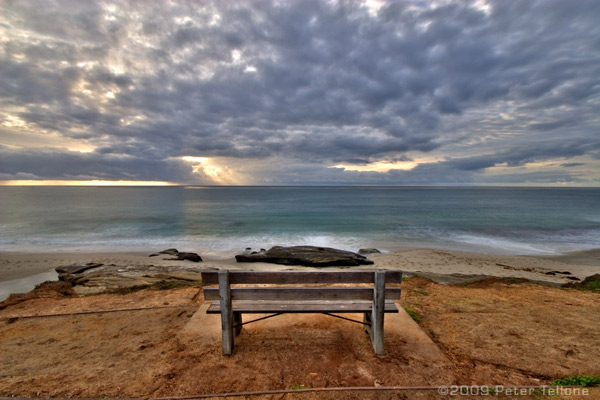
\includegraphics[width=0.6\textwidth]{example}
    \caption{HDR-Bild mit bereits angewandtem \gls{Tone-Mapping}-Verfahren \cite{tellone}}
    \label{fig:teezer}
  \end{center}
\end{figure}

Die Verwendung von \gls{HDR}-Bildern kann diese Problematik beheben. Ziel ist es, mehr Farben und Details in unterschiedlichen Bildbereichen sichtbar zu machen. Um dies zu ermöglichen, erhöht man bei \gls{HDR}-Bildern den \gls{Dynamikumfang} des Bildbereiches. Dazu ist jedoch eine andere Form der Repräsentation des Bildes notwendig (sog. \glspl{Radiance Map}).

%------------------------------------------------------------------------------------------------------------
\section{Prinzip}

Das menschliche Auge kann in einer täglichen Szene einen \gls{Dynamikumfang} im Bereich von 1:10.000 wahrnehmen \cite{Fairchild04theicam}. Dieser Umfang liegt weit über den herkömmlichen Werten eines normalen Kamera-Sensors. In der \autoref{tab:illumination} sind verschiedene Dynamikumfänge (und die damit zusammenhängenden Belichtungsstärken) aufgelistet. 
Um mit \gls{HDR}-Bildern einen höheren \gls{Dynamikumfang} darstellen zu können, müssen mehr Informationen als über den herkömmlichen Weg beschaffen werden. Dazu werden entweder mehrere Bilder mit verschiedenen Belichtungszeiten zu einer \gls{Radiance Map} kombiniert oder es werden spezielle Kamera-Sensoren eingesetzt, welche in der Lage sind eine höhere Dichte an Bildinformationen (z.B. große Helligkeitsunterschiede) aufzunehmen \cite{Yang99a640}. 


\begin{table}[b]
  \begin{center}
    \begin{tabular}{ccc}
	\toprule
	Umgebung & Belichtungsstärke ($cd/m^2$)\\ \midrule
	Sternenhimmel & $10^{-3} $\\	
	Mondschein & $10^{-1} $\\	
	Innenraum Beleuchtung & $10^{2} $\\	
	Sonnenlicht & $10^{5} $\\	
	\midrule
	Herkömmliche Monitore & $10^{2} $\\	
	\bottomrule
    \end{tabular}
    \caption{Belichtungsstärken in verschiedenen Umgebungen \cite[S.~6]{Reinhard}}
    \label{tab:illumination}
  \end{center}
\end{table}



Der hier verwendete Begriff \enquote{\gls{Dynamikumfang}} beschreibt das Verhältnis zwischen dem hellsten und dunkelsten Pixel im Bild. Um Ausreißern ein geringeren Einfluss zu geben und die Messung robuster zu machen, werden manchmal auch Quantile verwendet, wodurch Rauschen in der Eingabe weniger stark gewichtet wird. Bei Bildschirmen wird hingegen unter dem \gls{Dynamikumfang} das Verhältnis zwischen der maximalen und minimalen Leuchtkraft verstanden \cite[S.~4]{Reinhard}.


Nach der Vorstellung des Prinzips von \gls{HDR}-Bildern folgt nun eine kurze Auflistung von möglichen Anwendungsgebieten.

%------------------------------------------------------------------------------------------------------------

\section{Anwendungsgebiet und Geschichte}

Die Möglichkeiten des Einsatzes von \gls{HDR}-Bildern sind vielfältig. Die nachfolgende Liste umfasst einige der Gebiete, in denen diese Technologie eingesetzt wird oder werden kann \cite[S.~87f]{Reinhard}.

\begin{description}

\item[Digitale Fotografie:] Die verschiedenen Kamera-Hersteller tendieren zu sog.  \enquote{aufnahmeabhängigen Daten}. In diesen sind häufig mehr Bildinformationen enthalten. Dabei handelt es sich bei verschiedenen Herstellern in der Regel um verschiedene \acrfull{RAW}, die meist nicht kompatibel sind. 

\item[Satellitenbilder:] Satellitenbilder beinhalten in aller Regel sehr viel mehr Informationen als nur den sichtbaren Bereich des Lichtspektrums. \gls{HDR}-Bilder sind hier von Bedeutung, da sie multispektrale Aufnahmen ermöglichen.

\item[Visualisierungen und Rendering:] \gls{HDR}-Bilder wurden vermutlich zuerst in Render-Engines von Visualisierungen (Computer-Spiele, medizinische Visualisierungen und Simulationen, etc.) eingesetzt. Bei manchen Anwendungen ist es insbesondere für Reflektionen wichtig, auch nicht sichtbare Frequenzen bei Berechnungen mit einzubeziehen, da diese durch Interferenzen wieder sichtbar werden können und somit der Detailgrad steigt.

\item[Bildbearbeitungssoftware:] Die großen Bildbearbeitungsanwendungen bieten mittlerweile in der Regel ebenfalls die Bearbeitung und Generierung von \gls{HDR}-Bildern an (z.B. Adobe Photoshop\footnote{\url{http://adobe.com/photoshop}}, Photogenics\footnote{\url{http://www.cinepaint.org}} und Photomatix\footnote{\url{http://www.hdrsoft.com/download.html}}).

\item[Medizin:] In der Endoskopie besteht ein großer Bedarf an hoch auflösenden \gls{CMOS} Bildsensoren. Diese können immer bessere Aufnahmen aus dem Inneren des Körpers liefern und ermöglichen der Medizin große Fortschritte. Solche Sensoren können bereits in der Größe eines Streichholzkopfes einen Kontrastverhältnis von mehr als $10^7:1$ (179 dB) erreichen \cite{Klingler_Richter_Strobel_2006}.

\item[Virtual Reality:] In Anwendungen, bei denen sich der Benutzer in einem virtuellen Raum bewegt, wird die Wahrnehmung zunehmend wichtig. Auch hier spielen deshalb hohe Dynamikumfänge eine besondere Rolle. In diesem Bereich ist es besonders wichtig, gute Kompressions-Algorithmen für \gls{HDR}-Bilder zu entwickeln, um eine schnelle Übertragung zu gewährleisten. Auch beim Platzieren von synthetischen Objekten in realen Szenen können \gls{HDR}-Bilder eingesetzt werden, um dem Betrachter eine noch \enquote{realere} Szene zu suggestieren \cite{Debevec:2008:RSO:1401132.1401175}.
\end{description}


Um \gls{HDR}-Bilder in diesen Bereichen verwenden zu können müssen diese zunächst erzeugt werden. Im nachfolgenden Abschnitt werden drei verschiedene Möglichkeiten dazu vorgestellt.


%------------------------------------------------------------------------------------------------------------
\section{Bilderzeugung}
\label{sec:bilderzeugung}
Für die Erstellung von \gls{HDR}-Bildern gibt es unterschiedliche Möglichkeiten. Dabei muss jedoch zwischen echten \gls{HDR}-Bildern und Pseudo-\gls{HDR}-Bildern unterschieden werden. Im Nachfolgenden werden die verschiedenen Verfahren kurz beschrieben. Der Fokus liegt dieser Arbeit liegt auf dem letzten Verfahren, der \nameref{sub:belichtungsreihe}, da dieses auch im Ausgangsverfahren von Debevec und Malik verwendet wird.


\subsection{Pseudo-\gls{HDR}-Bilder}
Bei Pseudo-\gls{HDR}-Bildern handelt es sich um eine einfache Fusion von Bildreihen. Deswegen werden diese Verfahren auch Exposure Blending oder Exposure Fusion genannt. Bei dieser Technologie geht es darum, mehr Details aus einer Belichtungsreihe von \acrshort{LDR}-Bildern (\acrlong{LDR} Bilder) zu generieren, ohne dabei ein \gls{HDR}-Bild zu erzeugen. Die Bilder der Belichtungsreihe werden dazu einfach fusioniert \cite{Jing_Hong_Zheng_Rahardja_2012}.

\subsection{HDR-Kameras} 
Diese speziellen Kameras verfügen über Bildsensoren, die von sich aus einen höheren Dynamikumfang aufnehmen können und dadurch die notwendigen Informationen in einer Aufnahme generieren können. Diese Spezial-Kameras sind jedoch noch sehr teuer und wenig verbreitet \cite[S. 95ff]{Bloch2012}. Digitale Spiegelreflex-Kameras bieten mittlerweile häufig ebenfalls einen \gls{HDR}-Modus an.

\subsection{HDR-Bildgenerierung aus einer Belichtungsreihe}
\label{sub:belichtungsreihe}
Um ein \gls{HDR}-Bild aus einer Belichtungsreihe zu erzeugen, braucht man zunächst eine Grundlage für das Bild. In diesem Verfahren werden mehrere Bilder der selben Szene mit unterschiedlichen Belichtungszeiten fusioniert. Ziel der dabei verwendeten Algorithmen ist es, aus diesen Bildern ein \gls{HDR}-Bild zu erzeugen.

Um die Bilder später weiter zu verarbeiten, müssen diese jedoch zunächst registriert werden. Dieser Prozess beschreibt die gegenseitige Ausrichtung der Bilder einer Belichtungsreihe, sodass diese genau übereinander liegen. Dadurch werden Verschiebungen in den Belichtungsserien eliminiert, die z.B. durch das Bewegen der Kamera entstanden sind. Eine solche Registrierung ist aufgrund der verschiedenen Belichtungswerte der Aufnahmen häufig nicht oder nur schlecht über Kantendetektions-Verfahren möglich, da diese Merkmale unter den unterschiedlichen Belichtungen sehr stark variieren können.

Ein besserer Ansatz um Bilder zu registrieren ist der \gls{MTB} Ansatz (siehe \autoref{subsec:MTB}), da dieser ohne Kantendetektions-Verfahren auskommt. In den nachfolgenden Vergleichen und in der Implementierung wurde auf ein solches darauf verzichtet, da nur bereits registrierte Bilder verwendet werden.


Die so erstellten \gls{HDR}-Bildern sollen nun auch gespeichert werden können. Das nachfolgende Kapitel beschäftigt sich deshalb mit der Kodierung, Komprimierung und Abspeicherung von \gls{HDR}-Bildern.



%------------------------------------------------------------------------------------------------------------
\section{Bildformate und -speicherung}

Für die Abspeicherung der \gls{HDR}-Bilder werden in \autoref{tab:formats} die drei gängigsten Formate mit den dazu gängigen Kodierungen verglichen \cite[S.~89]{Reinhard}. Die Speicherung der erzeugten Daten war kein zentraler Bestandteil der vorliegenden Arbeit und wurde deshalb bei der Realisierung nicht berücksichtigt. Dennoch sollen hier die bekanntesten Kodierungen zur Abspeicherung vorgestellt werden.


\begin{table}[H]
  \begin{center}
    \small
    \begin{tabularx}{\textwidth}{l|XXXX}
	\toprule
	Format & Kodierung & Kompression & Metadaten & Lizenz \\
	\midrule
	HDR & RGBE & Laufl"angen-\newline kodierung & Kallibrierung, \newline Farbraum & Open source\newline software (\textit{Radiance})\\
	& XYZE & Laufl"angen-\newline kodierung & + benutzerdef.\newline Daten & \\
	\midrule
	TIFF & IEEE RGB & keine & Kallibrierung, \newline Farbraum & Public domain \newline library (\textit{libtiff})\\
	& LogLuv24 & keine &+ Registrierung \newline+ benutzerdef.\newline Daten& \\
	& LogLuv32 & Lauflängen-\newline kodierung & & \\
	\midrule
	EXR & Half RGB & Wavelet, ZIP & Kallibrierung, \newline Farbraum \newline+ Fensterfunktion \newline+ benutzerdef.\newline Daten & Open source library (\textit{OpenEXR})\\
	\bottomrule
    \end{tabularx}
    \normalsize
    \caption{\textit{HDR-Bildformate} --- Die verbreitetsten Formate und ihre Eigenschaften in der Übersicht \cite[S.89]{Reinhard}.}
    \label{tab:formats}
  \end{center}
\end{table}


\subsection{RGBE -- Das .hdr Format}

Dieses Datei-Format wurde ursprünglich unter den Dateiendungen \texttt{.hdr} und \texttt{.pic} eingeführt. Abgesehen von den Metadaten (wie z.B. Bildgröße, Ausrichtung, notwendige Angaben zur verwendeten Kodierung, etc.) wird jeder Bildpunkte mit 32-Bit dargestellt, die sich auf die Kanäle für Rot, Grün und Blau sowie einen Exponenten verteilen. Die Darstellung der Kanäle zusammen mit dem Exponenten führt zu einer Vergrößerung des Dynamikbereiches \cite[S. 92]{Reinhard}.

\subsection{TIFF -- Gleitkomma Kodierung}
\label{sub:tiff}
Das Format \texttt{.tiff} enthält eine 32-Bit Kodierung pro Komponente (also 96-Bit für einen Bildpunkt). Dabei werden die Bildpunkte mittels Fließkommazahlen dargestellt \cite{adobe:tiff}. Dieser Standard unterstützt bereits eine sehr hohe Genauigkeit. Dazu benötigt dieses Dateiformat im Vergleich zu anderen jedoch am meisten Speicherplatz. Allerdings lässt sich damit auch eine nahezu verlustfreie Abspeicherung von \gls{HDR}-Bildern erreichen. Im Standard von 1992 wurde auf jede Form der Komprimierung verzichtet \cite[S. 93]{Reinhard}. Dieser kann jedoch um verschiedene Kompressionsverfahren erweitert werden. \texttt{LogLuv} ist beispielsweise ein solches, bei dem die Werte logarithmisch skaliert und quantisiert werden \cite{logluv}. 


\subsection{EXR -- EXtended Range Format}

Dieses Format wurde 2002 veröffentlicht\footnote{\url{www.openexr.com}} und basiert ebenfalls auf der Speicherung von Fließkommazahlen. Es existiert eine Variante bei der nur 16 Bit (Hälfte der normalen Anzahl) für das Speichern der Fließkommazahlen verwendet wird: ein Bit für das Vorzeichen, fünf für den Exponenten und zehn für die Mantisse. Für diese Komprimierung sind Quantisierungsschritte von unter 0.1\% vorgesehen und damit für das menschliche Auge nicht erkennbar. Dadurch ist diese Kompression quasi verlustfrei durchführbar \cite[S. 97f]{Reinhard}.



%------------------------------------------------------------------------------------------------------------
\section{Bilddarstellung}
\label{subsec:ToneMapping}
Das Erstellen von \gls{HDR}-Bildern (siehe \autoref{sec:bilderzeugung}) erzeugt sog. \glspl{Radiance Map}. Dabei handelt es sich um eine Zuordnung der Bestrahlungsstärke durch das einfallende Licht zu jedem Bildpunkt einer Szene. 
Für die Darstellung dieser \glspl{Radiance Map} gibt es vereinzelt spezielle Hardware, die in der Lage ist den erweiterten Dynamikumfang darzustellen. Sehr viel häufiger kommen jedoch sog. \gls{Tone-Mapping} (dt.: Dynamikkompressions) Verfahren zum Einsatz. Diese stellen ein HDR-Bild durch eine andere Skalierung des Bildbereichs als herkömmliche Bilddateien dar. 
 
 Der Kerngedanke beim \gls{Tone-Mapping} besteht darin, einen geeigneten Weg für die Zuordnung von Bildpunkten aus dem \gls{HDR}-Bild in das \gls{LDR} Bild zu finden \cite[S. 145]{Bloch2012}. Diese Zuordnungsfunktionen nennen sich \gls{Tone-Mapping}-Operatoren und können generell in zwei Kategorien unterschieden werden. Die globalen Operatoren (siehe \autoref{sub:tone:global}) bearbeiten alle Bildpunkte gleich, während die lokalen Operatoren (siehe \autoref{sub:tone:local}) Informationen aus der Umgebung in die Berechnung an jedem Bildpunkt mit einbeziehen.
 

 \subsection{Globale \gls{Tone-Mapping}-Operatoren}
\label{sub:tone:global}
Bei globalen \gls{Tone-Mapping}-Operatoren wird die gesamte Farbkurve (engl. tone curves) modifiziert. Bei dieser Zuordnung handelt es sich um eine Korrelation zwischen Eingabe (\gls{HDR}-Bild) und Ausgabe (\gls{LDR}-Bild), die die Umrechnung der Belichtungsstärke in Farbwerte angibt. Die Veränderungen durch den \gls{Tone-Mapping}-Operator können auf den verschiedenen Farbkanälen unterschiedlich sein. Auch die Berechnung der modifizierten Kurve kann sich aufgrund des Bildes ändern \cite[S. 146]{Bloch2012}. 

Es bestehen viele verschiedene Ansätze für globale \gls{Tone-Mapping}-Operatoren, die unterschiedliche Vor- und Nachteile aufweisen.
In dieser Arbeit wurde lediglich der \gls{Tone-Mapping}-Operator von Reinhard et al. \cite{ReinhardToneMapper} implementiert und verwendet. Dabei handelt es sich um die vereinfachte Form des komplexeren lokalen Operators, der im gleichen Artikel veröffentlicht wurde.
Hierzu wird zunächst der durchschnittliche Wert des Logarithmus aus der Helligkeit des Bildes $L_w(x,y)$ bestimmt. Dieser wird als charakteristischer Wert der Szene $\tilde{L}_w$ beschrieben. Anschließend werden die skalierten Helligkeiten des Bildes errechnet (siehe \autoref{eq:skaled:greyvalues}). Der Parameter $\alpha$ bestimmt die Lage des mittleren Grauwertes und hat in der Regel den Wert $0.18$. Daraus lässt sich dann der globale Operator in \autoref{eq:tonemapping:global} erstellen.
\begin{align}
\label{eq:skaled:greyvalues}
L(x,y) = \frac{\alpha}{\tilde{L}_w} L_w(x,y)\\
\label{eq:tonemapping:global}
L_d(x, y) =\frac{L(x,y)}{1+ L(x,y)}
\end{align}


\subsection{Lokale \gls{Tone-Mapping}-Operatoren}
\label{sub:tone:local}

Lokale \gls{Tone-Mapping}-Operatoren können bei der Zuordnung eines Wertes aus einem \gls{HDR}- in ein \gls{LDR}-Bild auch die lokale Umgebung eines jeden Bildpunktes berücksichtigen. Damit erreichen sie in sehr dynamischen Bildern bessere Ergebnisse und können mehr Details in Bildern hervorheben. Auch hier gibt es eine Vielzahl verschiedener Operatoren, die alle ihre Vor- und Nachteile haben. Da der Operator von Reinhard et. al \cite{ReinhardToneMapper} in verschiedenen Veröffentlichungen \cite{tone_mapper_1,tone_mapper_2} gut abgeschnitten hat, wird dieser verwendet.

Bei diesem handelt es sich um einen lokalen \gls{Tone-Mapping}-Operator, der dodging-and-burning (dt. abwedeln) zur Berechnung verwendet. Dieses Verfahren ist eine Technik, die aus der analogen Fotografie stammt. Dabei wird die Belichtungszeit in einzelnen Bereichen des Bildes verändert, um diese bei der Entwicklung des Filmmaterials differenziert zu behandeln. Die Wahl der einzelnen Bereiche wird im technischen Ansatz durch die Berechnung des lokalen Kontrastes im Bild umgesetzt, welche die Reichweite des Operators beeinflussen. Auf eine weitere Beschreibung des Verfahrens wird hier aus Gründen der Komplexität verzichtet.

Für den gesamten Prozess der Erstellung, Speicherung und Darstellung von \gls{HDR}-Bildern gibt es verschiedene Software, welche die einzelnen Schritte durchführen kann. Der folgende Abschnitt stellt einige dieser Anwendungen vor.
%------------------------------------------------------------------------------------------------------------
\section{Software zur Erstellung von HDR-Bildern}
\label{sec:software}
Herkömmlich Programme zur Bildbearbeitung (z.B. \texttt{Photoshop}\footnote{\url{http://adobe.com/photoshop}} oder \texttt{GIMP}\footnote{\url{http://www.gimp.org} mit Plugin \texttt{Exposure Blend} (\url{http://tir.astro.utoledo.edu/jdsmith/code/exposure_blend.php})}) unterstützen die Erzeugung von \gls{HDR}-Bildern aus einer Belichtungsserie recht gut. Es gibt in der Regel mehrere \gls{Tone-Mapping}-Operatoren, deren Parameter anschaulich verändert werden können. Diese trumpfen mit hohem Funktionsumfang, vielfältigen Einstellungsvarianten und der Möglichkeit der weiteren Bearbeitung auf.


\begin{figure}
  \begin{center}
    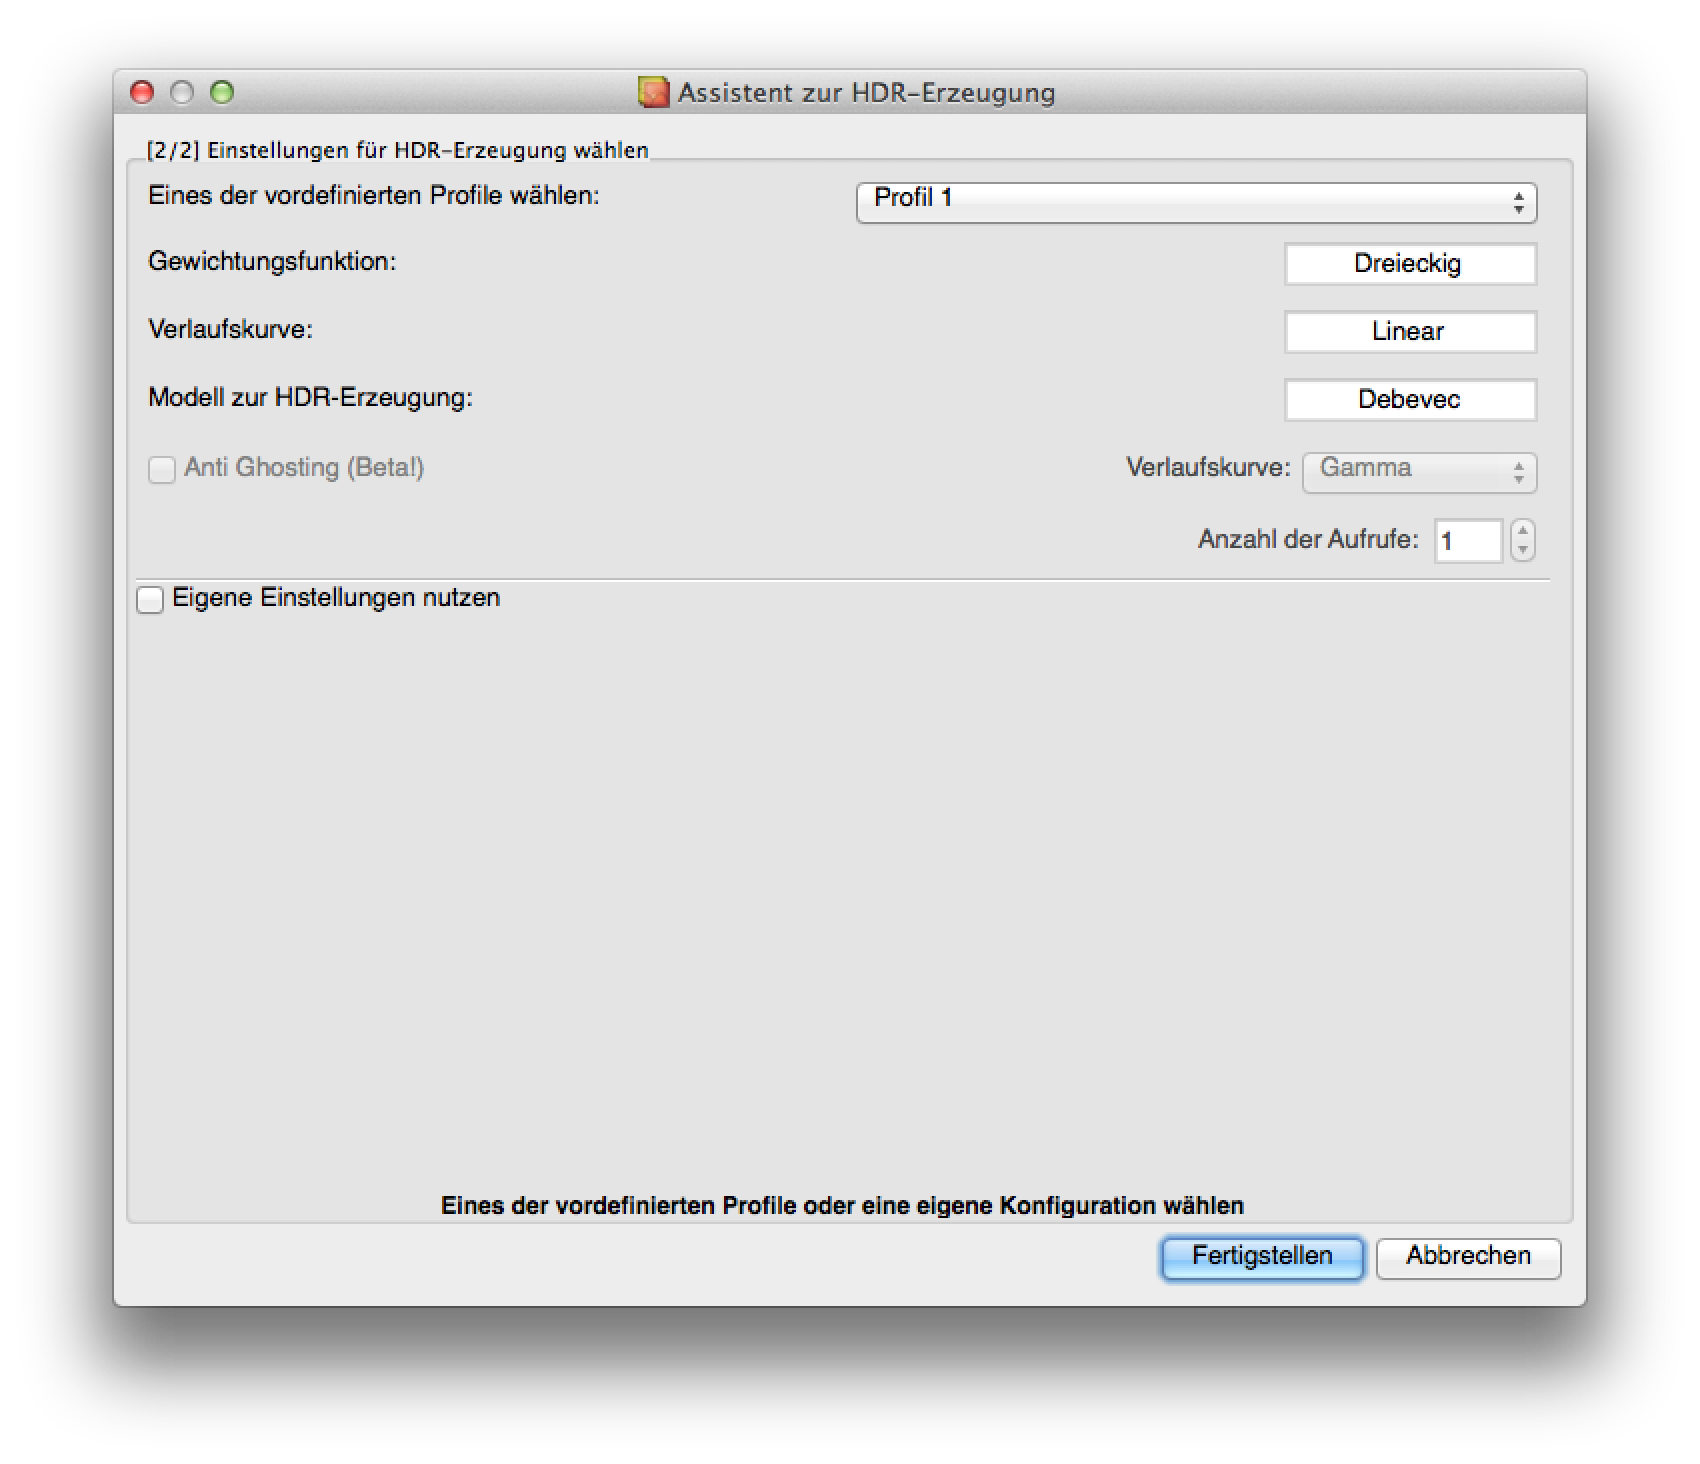
\includegraphics[width=0.8\textwidth]{Luminance}
    \caption{\textit{Erstell-Assistent von \texttt{Luminance HDR}} --- Auch hier wird intern der Algorithmus von Debevec und Malik verwendet.}
    \label{fig:luminance}
  \end{center}
\end{figure}

Darüber hinaus gibt es verschiedene Programme, die speziell auf die Erzeugung von \gls{HDR}-Bildern spezialisiert sind (z.B. \texttt{Photomatix}\footnote{\url{http://www.hdrsoft.com/de/}, kostenpflichtig} oder \texttt{Luminance HDR}\footnote{\url{http://qtpfsgui.sourceforge.net}, Freeware}). Der Funktionsumfang dieser Programme ist verhältnismäßig klein, führt auch Laien schnell zum Ziel, da (wie z.B. bei \texttt{Luminance HDR}, siehe \autoref{fig:luminance}) interaktive Assistenten den Benutzer bei der Erstellung anleiten. 

Als weitere Beispiele für \gls{HDR}-Software seien hier außerdem \texttt{Dynamic-Photo HDR}\footnote{\url{http://www.mediachance.com/hdri/index.html}, kostenpflichtig} und \texttt{HDR Darkroom}\footnote{\url{http://www.everimaging.com}, kostenpflichtig} genannt. Diese Programme verfügen über ein großes Portfolio von \gls{Tone-Mapping}-Operatoren und können sowohl realistische als auch sehr verfremdete \gls{HDR}-Bilder generieren. 

Ein wirklich einfaches Programm ist \texttt{Picturenaut}\footnote{\url{http://www.hdrlabs.com/picturenaut/}, Freeware}. Die Anzahl und der Funktionsumfang der implementierten \gls{Tone-Mapping}-Operatoren ist limitiert, jedoch liefert das Programm recht rasch realitätsgetreue Bilder.


